\providecommand{\main}{..}
\documentclass[../COS3712_Notes.tex]{subfiles}

\begin{document}
  \setcounter{chapter}{5}
  \chapter{From Vertices to Fragments}
    \begin{sidenote}{Textbook}
      In the textbook, this section corresponds to Chapter 8: From Geometry to Pixels.
    \end{sidenote}

    \concept{Clipping} involves eliminating objects that lie outside the viewing volume,
    and thus cannot be visible in the image.
    \concept{Rasterization} produces fragments from the remaining objects.
    These fragments can contribute to the final image.
    \concept{Hidden-surface~removal} determines which fragments correspond to objects
    that are visible, namely, those that are in the view volume and are not blocked
    from view by other objects closer to the camera.

    \section{Basic Implementation Strategies}
      \begin{figure}
        \begin{center}
          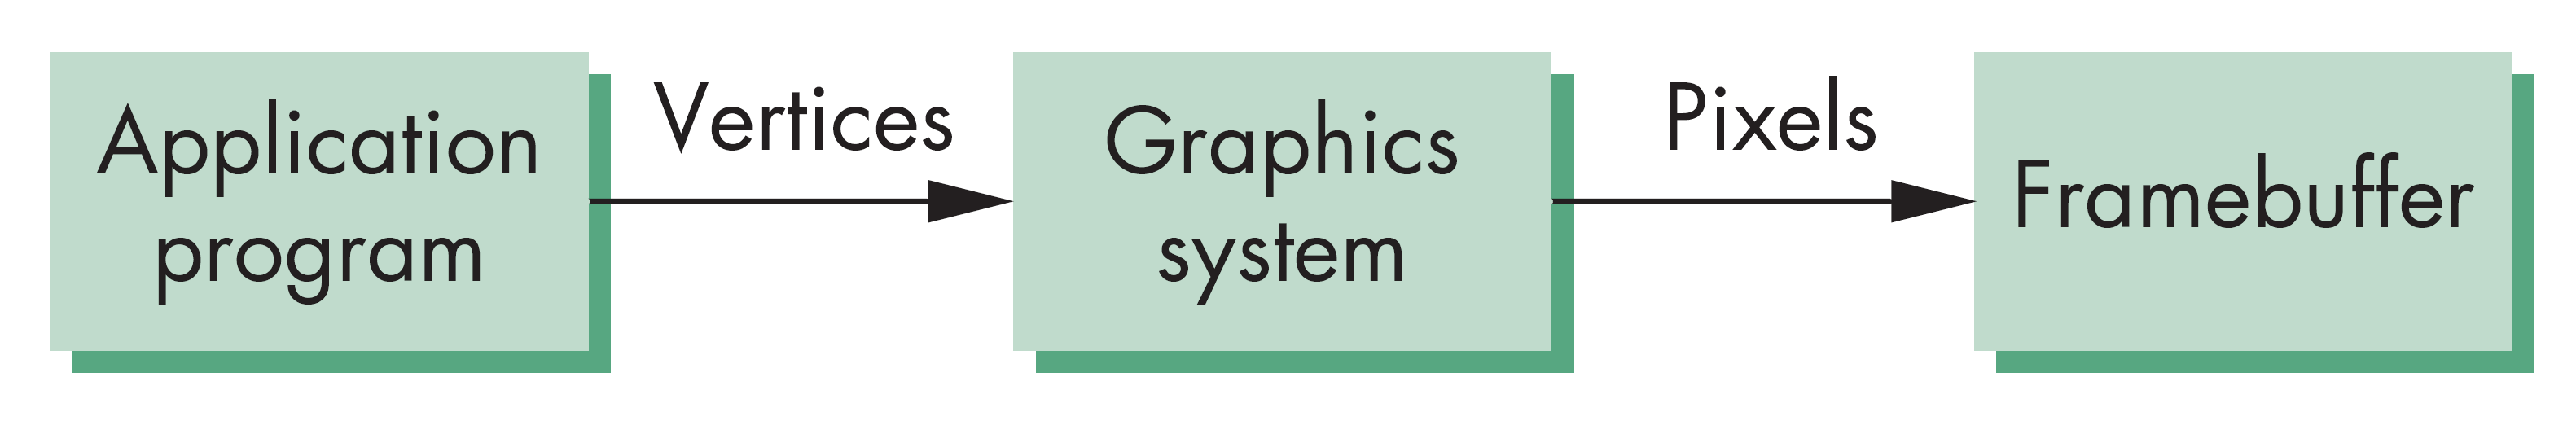
\includegraphics[width=0.7\textwidth]{\main/images/chapter06/graphics_process.png}
        \end{center}
        \caption{High-level view of the graphics process}
      \end{figure}

      In computer graphics, we start with an application program, and end with an image.
      We can consider this process as a black box whose inputs are the vertices and states
      defined in the program -- geometric objects, attributes, camera specifications --
      and whose output is an array of coloured pixels in the framebuffer.

      Within the black box, we must perform many tasks, including transformations,
      clipping, shading, hidden-surface removal, and rasterization of the primitives
      that can appear on the display.
      These tasks can be organised in a variety of ways, but regardless of the strategy
      we adopt, we must always do two things:
      \begin{enumerate}[nosep]
        \item We must pass every geometric object through the system, and
        \item we must assign a colour to every pixel in the colour buffer that is displayed.
      \end{enumerate}

      Suppose we think of what goes into the black box in terms of a single program
      that carries out the entire process.
      Because this program must assign a value to every pixel and must process every
      geometric primitive (and light source),
      we expect this program to contain at least two loops that iterate over these basic
      variables.
      The variable we choose to control the outer loop determines the flow of the entire
      implementation process.
      There are two fundamental strategies: the \concept{image-oriented} approach, and the
      \concept{object-oriented} approach.

      \begin{definition}{Object Oriented Approach}
        The outer loop iterates over the objects.

        A pipeline renderer fits this description.
        Vertices are defined by the program and flow through a sequence of modules that
        transforms them, colours them, and determines whether they are visible.

        After a polygon passes through geometric processing, the rasterization
        of this polygon can potentially affect any pixels in the framebuffer.

        Most implementations that follow this approach are based on construction of a
        rendering pipeline containing hardware or software modules for each of the tasks.
        Data (vertices) flow \emph{forward} through the system.

        In the past, the major limitations of the object-oriented approach were the
        large amount of memory required and the high cost of processing each object
        independently.
        Any geometric primitive that emerges from the geometric processing can potentially
        affect any set of pixels in the framebuffer.
        So, the entire colour buffer, and various other buffers, must be of the size of the
        display, and must be available at all times.

        Today, the main limitation of object-oriented implementations is that they cannot
        handle most global calculations.
        Because each geometric primitive is processed independently
        -- and in an arbitrary order --
        complex shading effects that involve multiple geometric objects,
        such as reflections,
        cannot be handled except by approximate methods.
        The major exception is hidden-surface removal, where the $z$-buffer is used to store
        global information.
      \end{definition}

      \begin{definition}{Image-Oriented Approach}
        The outer loop iterates over pixels, or rows of pixels called \concept{scan~lines},
        that constitute the framebuffer.

        For each pixel, we work \emph{backward}, trying to determine which geometric primitives
        can contribute to its colour.

        The advantages of this approach are that we need only limited display memory
        at any time and that we can hope to generate pixels
        at the rate and in the order required to refresh the display.
        Because the results of most calculations do not differ from pixel to pixel
        (or scan line to scan line),
        we can use this coherence in our algorithms by developing incremental forms
        for many of the steps in the implementation.

        The main disadvantage of this approach is that, unless we first build a data structure
        from the geometric data, we do not know which primitives affect which pixels.
        Such a data structure can be complex, and may imply that all the geometric data
        must be available at all times during the rendering process.
        For problems with very large databases, even having a good data representation
        may not avoid memory leaks.
        However, because image-space algorithms have access to all objects for each pixel,
        they are well suited to handle global effects, such as shadows and reflections.
      \end{definition}

      Within these two major categories specified by two loops, each may contain other loops.

\end{document}
